% Format teze zasnovan je na paketu memoir. Prilikom
% zadavanja klase memoir, navedenim opcijama se podešava
% veličina slova (12pt) i jednostrano štampanje (oneside).
\documentclass[12pt,oneside]{memoir}

% Paket koji definiše sve specifičnosti mastera Matematičkog fakulteta
\usepackage{matfmaster}

% Paket koji obezbeđuje ispravni prikaz ćiriličkih italik slova
\usepackage{cmsrb}

% Ostali paketi koji se koriste u dokumentu
\usepackage{amsmath} % matematika (matrice)
\usepackage{CJKutf8} % japanski jezik (CJK)
\usepackage[ruled]{algorithm2e} % algoritmi
\usepackage{nicematrix} % lepe matrice (mape)
\usepackage[strings]{underscore} % donja crta

% Učitavanje slika iz posebnog direktorijuma
\graphicspath{{../slike}}

% Komanda za ispis (npr. caption) u dva reda
\newcommand{\dvareda}[2][c]{\begin{tabular}[#1]{@{}c@{}}#2\end{tabular}}

% Komanda za rad sa problemima na srpskom
\newenvironment{problem}[1][!ht]
{\renewcommand{\algorithmcfname}{Проблем}
\begin{figure}[!ht]
\centering
  \begin{minipage}{.94\linewidth}
	\begin{algorithm}[#1]%
  }{\end{algorithm}
  \end{minipage}
\end{figure}}

% Datoteka sa literaturom u BibTex tj. BibLaTeX/Biber formatu
\bib{HMM-u-bioinformatici}

% Ime kandidata na srpskom jeziku (u odabranom pismu)
\autor{Лазар М. Васовић}
% Naslov teze na srpskom jeziku (u odabranom pismu)
\naslov{Скривени Марковљеви модели (\textit{HMM}) у биоинформатици}
% Godina u kojoj je teza predana komisiji
\godina{2021}
% Ime i afilijacija mentora (u odabranom pismu)
\mentor{др Јована \textsc{Ковачевић}, доцент\\ Универзитет у Београду, Математички факултет}
% Ime i afilijacija prvog člana komisije (u odabranom pismu)
\komisijaA{... ... \textsc{...}, ...\\ ..., ...}
% Ime i afilijacija drugog člana komisije (u odabranom pismu)
\komisijaB{... ... \textsc{...}, ...\\ ..., ...}
% Datum odbrane (obrisati ili iskomentarisati ako nije poznat)
\datumodbrane{септембар 2021.}

% Apstrakt na srpskom jeziku (u odabranom pismu)
\apstr{%
...
}

% Ključne reči na srpskom jeziku (u odabranom pismu)
\kljucnereci{биоинформатика, скривени Марковљеви модели (\textit{HMM})}

\begin{document}
\begin{CJK}{UTF8}{ipxm}
% ====================================================================
% Uvodni deo teze
\frontmatter
% ====================================================================
% Naslovna strana
\naslovna
% Strana sa podacima o mentoru i članovima komisije
\komisija
% Strana sa podacima o disertaciji na srpskom jeziku
\apstrakt
% Sadržaj teze
\tableofcontents*

% ====================================================================
% Glavni deo teze
\mainmatter
% ====================================================================

% ------------------------------------------------------------------------------
\chapter{Увод}
% ------------------------------------------------------------------------------
Биоинформатика је интердисциплинарна област која се бави применом рачунарских технологија у области биологије и сродних наука, са нагласком на разумевању биолошких података. Кључна особина јој је управо поменута мултидисциплинарност, која се представља дијаграмом са слике \ref{fig:venn}.

\begin{figure}[!ht]
  \centering
  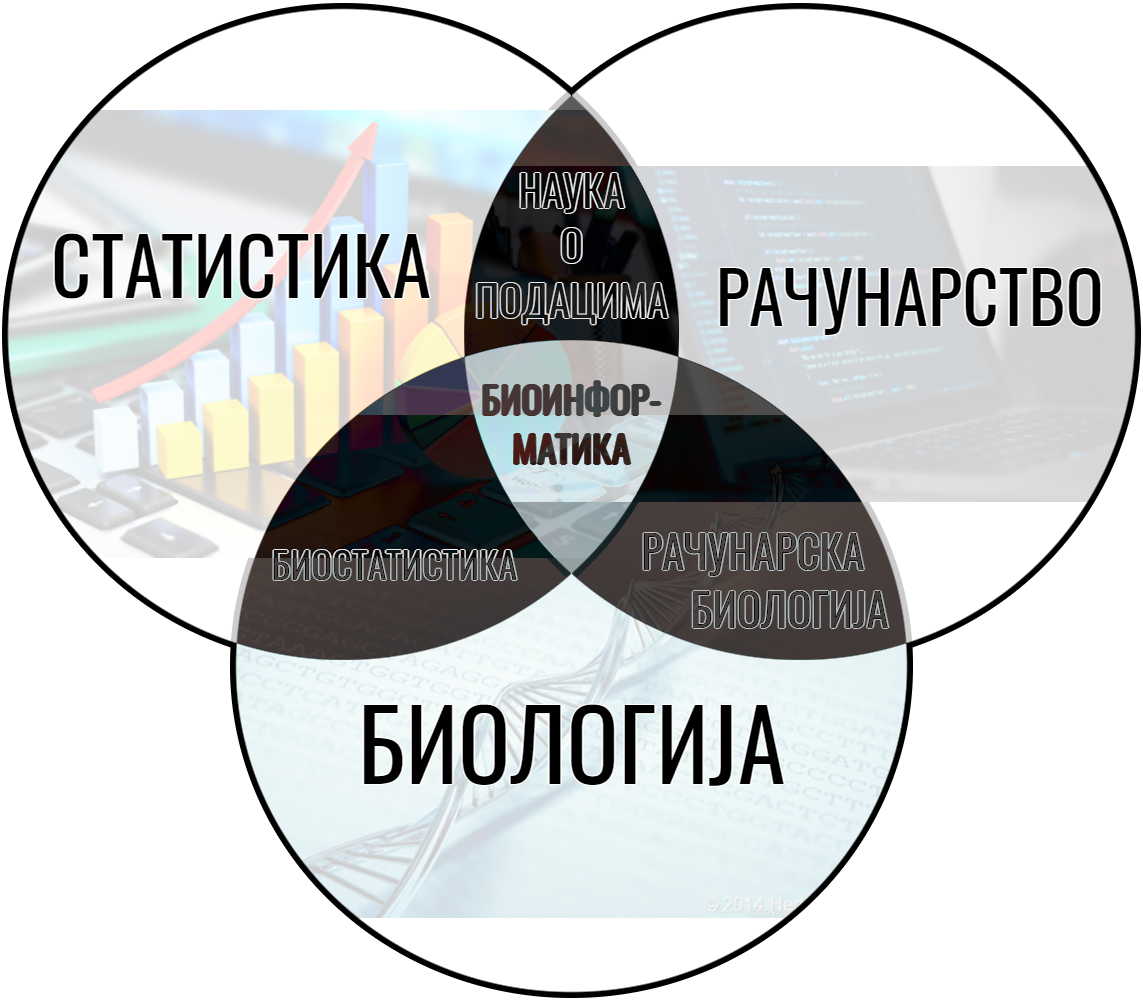
\includegraphics[width=.75\textwidth]{bioinformatika.png}
  \caption{Венов дијаграм интердисциплинарности\cite{venn}}
  \label{fig:venn}
\end{figure}

Овако представљена, биоинформатика је заправо спој статистике, рачунарства и биологије -- сва три истовремено -- по чему надилази појединачне спојеве: биостатистику, науку о подацима и рачунарску биологију. Конкретно, статистички (математички) апаратат служи за рад са подацима, рачунарске технологије тај апарат чине употребљивијим, док биологија даје потребно доменско знање (разумевање) за рад са биолошким и сродним подацима. Иако се може рећи да је биоинформатика, у савременом смислу представљеном приказаним дијаграмом, релативно млада наука, брзо је постала популарна и многи су јој посветили пажњу или се њоме баве\cite{fauziyyah2019, cmero2015, ufpr}.

Међу познатим личностима из овога домена издвајају се научници Филип Компо (\textit{Phillip Compeau}) и Павел Певзнер (\textit{Pavel Pevzner}), аутори књиге \textit{Bioinformatics Algorithms: An Active Learning Approach}. Прво издање књиге изашло је 2014. године, а друго већ наредне, у два тома. Актуелно, треће издање, издато је 2018. године, у једном тому. Захваљујући динамичном и активном приступу биолошким проблемима и њиховим информатичким решењима, као и многим додатним материјалима за учење, књига се користи као уџбеник на више од сто светских факултета\cite{ba}. Међу њима је и Математички факултет Универзитета у Београду, односно на њему доступни мастер курс Увод у биоинформатику, а делови књиге користе се и у настави повезаног мастер и докторског курса Истраживање података у биоинформатици\cite{matf}.

Актуелна иницијатива на нивоу курса Увод у биоинформатику јесте израда електронског уџбеника, заснованог на поменутој књизи. Идеја је да заинтересовани студенти као мастер рад обраде по једно поглавље књиге, при чему обрада укључује писање текста на српском језику, али и имплементацију и евентуалну визуелизацију свих или макар већине пратећих алгоритама. Овај рад настао је управо у склопу представљене иницијативе, међу првима.

Уџбеник кроз једанаест глава обрађује разне теме које су занимљиве у оквиру биоинформатике: почетак репликације (алгоритамско загревање), генске мотиве (рандомизовани алгоритми), асемблирање генома (графовски алгоритми), секвенцирање антибиотика/пептида (алгоритми грубе силе), поређење и поравнање геномских секвенци (динамичко програмирање), блокове синтеније (комбинаторни алгоритми), филогенију (еволутивна стабла), груписање гена (кластеровање), проналажење шаблона (префиксна и суфиксна стабла), откривање гена и мутација секвенце (скривени Марковљеви модели), напредно секвенцирање пептида (рачунарска протеомика). Циљ овог рада је обрада десетог поглавља, заснованог на скривеним Марковљевим моделима\cite{compeau2015}.

Скривени Марковљев модел (у наставку углавном скраћено \textit{HMM}, према енгл. \textit{Hidden Markov Model}), укратко, представља статистички модел који се састоји из следећих елемената: скривених стања ($x_i$), опсервација ($y_i$), вероватноћа прелаза ($a_{ij}$), полазних ($\pi_i$) и излазних вероватноћа ($b_{ij}$), по примеру са слике \ref{fig:hmm}. \textit{HMM} се тако може схватити као коначни аутомат, при чему стања задржавају уобичајено значење, док вероватноће прелаза описују колико се често неки прелаз реализује. Полазне вероватноће одређују почетно стање. Овакав аутомат допуњује се идејом да свако стање са одређеном излазном вероватноћом емитује (приказује) неку опсервацију. Штавише, најчешће су само опажања и позната у раду са \textit{HMM}, док се позадински низ стања погађа ("предвиђа"), па се управо зато стања и модели називају скривеним\cite{stamp2021}.

\begin{figure}[!ht]
  \centering
  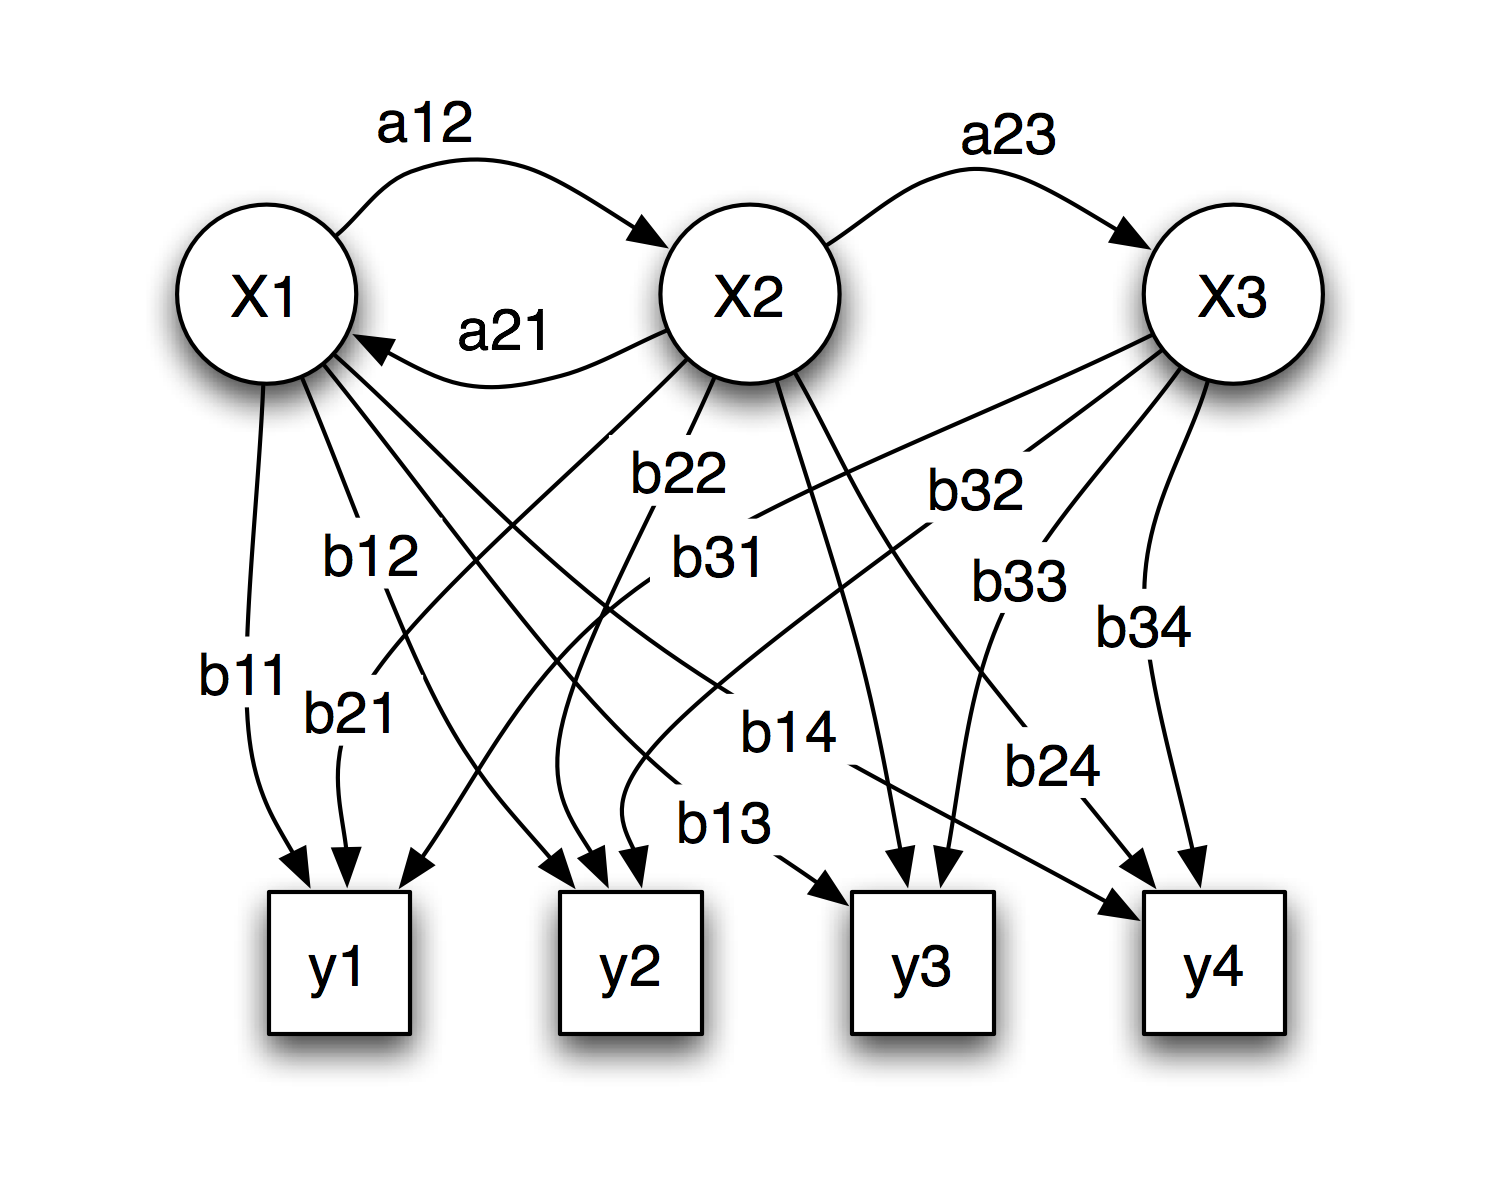
\includegraphics[width=.75\textwidth]{hmm.png}
  \caption{Једноставан пример скривеног Марковљевог модела\cite{hmm}}
  \label{fig:hmm}
\end{figure}

У претходном пасусу су, наравно, скривени Марковљеви модели представљени малтене само концептуално, на високом нивоу. У наставку су, међутим, они постепено уведени, заједно са мотивацијом за њихову употребу у виду биолошких проблема који се њима решавају. Према идеји електронског уџбеника, излагање прати књигу \textit{Bioinformatics Algorithms: An Active Learning Approach}, а имплементирани су сви пратећи алгоритми. Резултујући уџбеник са \textit{Python} кодовима, у виду \textit{Jupyter} свезака, доступан је на \textit{GitHub}-у\cite{vasovich2021}.

% ------------------------------------------------------------------------------
\chapter{Мотивација}
% ------------------------------------------------------------------------------
За почетак, изложена је мотивација за употребу скривених Марковљевих модела у биоинформатици. Конкретно, представљена су два важна биолошка проблема која се њима могу решити и пратећи појмови из домена, као и једна историјски мотивисана вероватносна мозгалица. Ова глава, дакле, покрива прву петину обрађеног поглавља \textit{Chapter 10: Why Have Biologists Still Not Developed an HIV Vaccine? -- Hidden Markov Models}, и то тачно следеће поднаслове: \textit{Classifying the HIV Phenotype}, \textit{Gambling with Yakuza}, \textit{Two Coins up the Dealer’s Sleeve}, \textit{Finding CG-Islands}, као и највећи део додатка из \textit{Detours}.

% Classifying the HIV Phenotype
\section{Погађање фенотипа}
\textit{HIV} је вирус хумане имунодефицијенције, један од најпознатијих вируса, који заражава људе широм света. Својим дугорочним деловањем доводи до смртоносног синдрома стечене имунодефицијенције, познатијег као сида или ејдс. Мада поједини аутори распрострањеност \textit{HIV}-а називају пандемијом, Светска здравствена организација означава је као "глобалну епидемију"\cite{who}.

Постојање \textit{HIV}-а званично је потврђено почетком осамдесетих година двадесетог века, мада се претпоставља да је са примата на људе прешао знатно раније. Недуго по овом открићу, тачније 1984, из америчког Министарства здравља и услуга становништву најављено је да ће вакцина бити доступна кроз наредне две године. Иако до тога није дошло, председник Бил Клинтон је 1997. потврдио да "није питање \textit{да ли} можемо да произведемо вакцину против сиде, већ је просто питање \textit{када} ће до тога доћи". Вакцина, међутим, ни данас није доступна, а многи покушаји су отказани након што се испоставило да кандидати чак повећавају ризик од инфекције код појединих испитаника.

Антивирусне вакцине најчешће се праве од површинских протеина вируса на који се циља, у нади да ће имунски систем, након вакцине, у контакту са живим вирусом знатно брже препознати протеине омотача вируса као стране и уништити их пре него што се вирус намножи у телу. \textit{HIV} је, међутим, карактеристичан по томе што врло брзо мутира, па су његови протеини изузетно варијабилни и није могуће научити имунски систем да исправно одреагује на све мутације. Штавише, може се десити да имунитет научи да исправно реагује само на једну варијанту вируса, а да реакција нема никаквог ефекта на остале варијанте. Овакав имунитет је лошији од имунитета који ништа не зна о вирусу, пошто не покушава да научи ништа ново, што је разлог већ поменуте ситуације да су код неких испитаника вакцине кандитати повећали ризик од заразе. Да ствар буде гора, \textit{HIV} брзо мутира и унутар једне особе, тако да је разлика у узорцима узетих од различитих пацијената увек значајна.

Када се све узме у обзир, као обећавајућа замисао за дизајн свеобухватне вакцине намеће се следећа идеја: идентификовати неки пептид који садржи најмање варијабилне делове површинских протеина свих познатих сојева \textit{HIV}-а и искористити га као основу вакцине. Ни то, међутим, није решење, пошто \textit{HIV} има још једну незгодну способност: уме да се сакрије процесом гликозилације. Наиме, протеини омотача су махон гликопротеини, што значи да се након превођења за њих могу закачити многобројни гликански (шећерни) ланци. Овим процесом долази до стварања густог гликанског штита, који омета имунски систем у препознавању вируса. Све досад изнето утиче на немогућност прављења прикладне вакцине у скоријем времену.

Чак и ван контекста вакцине, мутације \textit{HIV}-а прилично су занимљиве за разматрање. Конкретно, илустративно је бавити се \textit{env} геном, чија је стопа мутације 1--2 \% по нуклеотиду годишње. Овај ген кодира два релативно кратка гликопротеина који заједно граде шиљак (спајк) омотача, део вируса задужен за улазак у људске ћелије. Мање важан део шиљка је гликопротеин \textit{gp41} ($\sim$ 345 аминокиселина), док је важнији гликопротеин \textit{gp120} ($\sim$ 480 аминокиселина). О варијабилности другог говори чињеница да на нивоу једног пацијента, у кратком року, скоро половина аминокиселина буде измењено позадинским мутацијама одговарајућег гена, као да је сасвим други протеин.

Ствари постају још занимљивије када се, поред генотипа вируса, разматра и његов фенотип. Примера ради, сваки вирус \textit{HIV}-а може се означити као изолат који ствара синцицијум или као изолат који га не ствара. Након уласка у људску ћелију, гликопротеини омотача могу да изазову спајање заражене ћелије са суседним ћелијама. Резултат тога је синцицијум -- нефункционална вишеједарна ћелијска (цитоплазматична) маса са заједничком ћелијском мембраном. Овакав изолат \textit{HIV}-а означава се као онај који ствара синцицијум и он се тим процесом знатно брже умножава, што даље значи да је опаснији и агресивнији, јер уласком у само једну ћелију убија многе друге у суседству. Одређивање тачног генотипа и погађање фенотипа важно је како би се пацијенту преписао најприкладнији коктел антивирусних лекова.

Испоставља се да је примарна структура гликопротеина \textit{gp120} важан суштински генотипски предиктор фенотипа \textit{HIV}-а. Наиме, узимајући у обзир само низ аминокиселина које чине \textit{gp120}, може се направити једноставан класификатор који погађа да ли проучавани изолат ствара синцицијум или не. Конкретно, научник Жан Жак де Јонг је 1992. анализирао вишеструко поравнање такозване \textit{V3} петље, издвојеног региона у оквиру \textit{gp120}, и формулисао правило 11/25\cite{jong1992}. Према том правилу, сој \textit{HIV}-а највероватније ствара синцицијум уколико му се на 11. или 25. позицији у \textit{V3} петљи налазе аминокиселине аргинин (\textit{R}) или лизин (\textit{K}). Пример мотива \textit{V3} петље дат је на слици \ref{fig:motif}. Приметно је да су управо 11. и 25. позиција међу најваријабилнијим, те да удео критичних \textit{R} и \textit{K} на њима није претерано велик. Наравно, на фенотип утичу и многе друге позиције унутар \textit{gp120} и других протеина.

\begin{figure}[!ht]
  \centering
  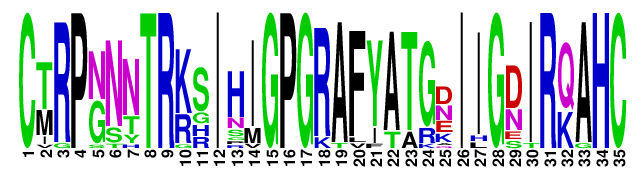
\includegraphics[width=.75\textwidth]{motif.png}
  \caption{Мотив \textit{V3} петље из \cite{compeau2015} генерисан помоћу \cite{weblogo}}
  \label{fig:motif}
\end{figure}

За крај и поенту уводне приче о \textit{HIV}-у, остаје неразрешен још један веома значајан проблем. Како би се уопште разматрало предвиђање фенотипа на основу примарне структуре \textit{gp120}, неопходно је прво доћи до прецизног вишеструког поравнања различитих секвенци аминокиселина. Прво, поравнање мора бити хируршки прецизно, јер нпр. само једна грешка доводи до погрешног податка која вредност је на 11. и 25. позицији \textit{V3} петље. Следеће, неопходно је адекватно обрадити инсерције и делеције, што су врло честе мутације \textit{HIV}-а у многим регионима генома. На крају, потребно је на прави начин оценити квалитет поравнања, нпр. коришћењем различитих матрица скора за сваку појединачну позицију. Ово је донекле могуће урадити коришћењем техника представљених у петом поглављу (\textit{Chapter 5: How Do We Compare DNA Sequences? -- Dynamic Programming}), али уз два главна проблема: алгортми динамичког програмирања су високе сложености и са мање слободе код скорова, а притом не пресликавају најбоље суштину биолошког проблема класификације фенотипа у алгоритамски проблем (фале кораци након поравнања). Постоји, дакле, потреба за новом формулацијом која обухвата све што је потребно за статистички потковано поравнање секвенци.

% Finding CG-Islands
\section{Потрага за генима}
Познато је да геном чини тек мали део \textit{DNA} секвенце. Другим речима, \textit{DNA} добрим делом не кодира протеине. Стога је један од важних биолошких проблема управо проналажење места на којима се гени налазе. Прецизније, тражи се место где њихово преписивање (транскрипција) започиње.

Почетком двадесетог века, Фибус Левин открио је да \textit{DNA} чине четири нуклеотида\cite{levene1910}, чији су главни део азотне базе: аденин (\textit{A}), цитозин (\textit{C}), гуанин (\textit{G}) и тимин (\textit{T}). У то време, међутим, није била позната тачна структура наследног материјала, штo је двострука завојница, коју су пола века касније открили Вотсон и Крик\cite{watson1953}. Левин је, стога, сматрао да \textit{DNA} носи информације једнаке било којој четворословној азбуци, а додатно и да је удео сваког од четири нуклеотида једнак. Занимљивост је да овај упрошћени модел одговара стању у савременој биоинформатици -- \textit{DNA} се углавном и посматра као секвенца нуклеотида, односно ниска над азбуком \{\textit{A}, \textit{C}, \textit{G}, \textit{T}\}.

Открићем тачне структуре допуњена је теза о једнаком уделу нуклеотида. Како су нуклеотиди на супротним ланцима упарени, њихов удео јесте врло сличан када се посматра целокупна \textit{DNA}. То, међутим, није случај када се посматра само један ланац, што је уобичајено у генетици и биоинформатици. Примера ради, удео гуанина и цитозина, који чине један базни пар, код људи је 42 \%, што је ипак статистички значајно мање од пола. На вишем нивоу гранулације, у случају да се посматрају само по две суседне базе, испоставља се да динуклеотиди \textit{CC}, \textit{CG}, \textit{GC}, \textit{GG} узимају сасвим различите уделе. Конкретно, иако би се очекивало да, под претпоставком равномерне расподеле, сваки од њих узима удео 4--5 \%, динуклетид \textit{CG} чини само 1 \% људског генома. Све ово значи да је \textit{DNA} секвенца ипак нешто даље од случајне.

Поставља се питање зашто је удео \textit{CG} тако мали. Одговор, међутим, није комплексан, поготову ако се додатно примети да је удео \textit{TG} нешто виши од очекиваног, а посебно у регионима у којима је удео \textit{CG} изразито мали. Разлог томе лежи у метилацији, најчешћој измени која природно настаје унутар \textit{DNA}. Поједини нуклеотиди, наиме, могу бити нестабилни, па се на њих лако накачи метил група ($CH_3$). Међу најнестабилнијим управо је цитозин иза ког следи гуанин, дакле \textit{C} из \textit{CG}. Метиловани цитозин даље се често спонтано деаминује у тимин, чиме динуклеотид \textit{CG} лако постаје \textit{TG}. Свеукупни резултат је да се \textit{CG} глобално појављује веома ретко, а \textit{TG} нешто чешће.

Метилација мења експресију суседних гена. Експресија оних гена чији су нуклеотиди у великој мери метиловани често је потиснута. Иако је сам процес метилације важан у току ћелијске диференцијације -- доприноси неповратној специјализацији матичних ћелија -- она углавном није пожељна у каснијем добу. Хиперметилација гена повезана је са различитим врстама рака. Стога је метилација врло ретка око гена, што значи да је на тим местима \textit{CG} знатно чешће. Овакви делови \textit{DNA} називају се \textit{CG} острвима или \textit{CpG} местима. Разлика у уделу динуклеотида у некодирајућим и регионима богатим генима дата је кроз табелу \ref{tab:cg}. Разлика у уделу \textit{CG} наглашена је црвеном бојом.

\begin{table}[h!]
  \centering
  \caption{\dvareda{Удео динуклеотида у једном ланцу људског \textit{X} хромозома\\-- лево у регионима \textit{CG} острва, а десно ван њих\cite{compeau2015}}}
  \begin{tabular}{c | c c c c | c c c c}
   & A & C & G & T & A & C & G & T\\ \hline
  A & 0,053 & 0,079 & 0,127 & 0,036 & 0,087 & 0,058 & 0,084 & 0,061\\
  C & 0,037 & 0,058 & \textcolor{red}{0,058} & 0,041 & 0,067 & 0,063 & \textcolor{red}{0,017} & 0,063\\
  G & 0,035 & 0,075 & 0,081 & 0,026 & 0,053 & 0,053 & 0,063 & 0,042\\
  T & 0,024 & 0,105 & 0,115 & 0,050 & 0,051 & 0,070 & 0,084 & 0,084\\
  \end{tabular}
  \label{tab:cg}
\end{table}

Закључак је, дакле, да се проблем потраге за генима може свести на проналажење \textit{CG} острва. Наиван приступ решавању овог проблема јесте употреба клизајућег прозора. Могао би се узети прозор фиксне величине и померати кроз \textit{DNA} секвенцу. Они прозори са натпросечним уделом \textit{CG} били би кандидати за \textit{CG} острва. Остаје, међутим, питање како одредити добру величину прозора, али и шта радити када преклапајући прозори нуде различиту класификацију подниза. И овде би добро дошло статистички потковано решење.

% Gambling with Yakuza
% Two Coins up the Dealer’s Sleeve
\section{Коцкање са јакузама}
Јакузе су припадници истоимене криминалне организације, традиционалног синдиката организованог криминала. Савремене јакузе потичу од јапанских путујућих коцкара, који су били распрострањени у осамнаестом веку. Једна од најпознатијих игара коју су путујући коцкари организовали у својим импровизованим коцкарницама био је чо-хан (јап. 丁半, \textit{chō-han}), у дословном преводу "пар-непар"\cite{fletcher2017}. Игра је сасвим једноставна -- претеча јакуза (крупије) баца две коцкице, док се играчи кладе да ли ће збир бити паран или непаран. Игра је такође поштена -- једнако се остварују оба исхода парности.

До занимљивог тренутка долази када се из било ког разлога осетно више играча опклади на један од два могућа резултата. Тада би имало смисла да похлепни крупије, у жељи да заради (он узима проценат зараде победника), баца отежане коцкице, које ће са већом вероватноћом дати резултат који је добио мање опклада. Једноставности ради, уместо чо-хана је у наставку разматрана нешто простија игра бацања новчића. У њој крупије баца новчић, а играчи се кладе да ли ће пасти писмо или глава. Она је знатно лакша за анализу, а суштина је иста и доводи до статистички поткованог решења у претходним поднасловима изложених биолошких и сродних проблема.

Крупијева превара у овом случају могла би бити употреба отежаног новчића, код кога исходи нису равномерно расподељени. Нека је познато да крупије има два новчића: један праведан и један отежан тако да на главу пада трипут чешће него на писмо. Циљ је за одређени низ исхода одредити да ли је настао бацањем праведног или отежаног новчића. Пажљивијом анализом проблема, испоставља се да је питање вара ли крупије лоше формулисано. Наиме, оба новчића могу да произведу било који низ исхода, па тако нпр. и отежани новчић може константно да пада на писмо. Иако дефинитивно није могуће са сигурношћу утврдити који је новчић коришћен, могуће је нешто слично и често довољно добро -- одредити који је вероватније коришћен.

Конкретно, нека је упитни новчић бачен одређени број пута, при чему је добијен низ исхода. Вероватноће исхода ($H$ од енгл. \textit{heads} -- глава и $T$ од енгл. \textit{tails} -- писмо) код праведног ($F$ од енгл. \textit{fair} -- фер) и отежаног ($B$ од енгл. \textit{biased} -- пристрасан) новчића могу се исказати следећим формулама: $$P\{H | F\} = P\{T | F\} = \frac{1}{2}, P\{H | B\} = \frac{3}{4}, P\{T | B\} = \frac{1}{4}.$$ Како су бацања независни догађаји -- претходни исходи ни на који начин не утичу на наредне -- вероватноћа да $n$ бацања произведе низ исхода $x = x_1...x_n$, од којих је пало $k$ глава, јесте производ појединачних вероватноћа: $$P\{x\} = \prod_{i=1}^n P\{x_i\} = P\{H\}^k \cdot P\{T\}^{n-k}.$$ Због тога вероватноћа сваког низа исхода код праведног новчића износи: $$P\{x | F\} = \left(\frac{1}{2}\right)^k \left(\frac{1}{2}\right)^{n-k} = \frac{1}{2^n}.$$ С друге стране, вероватноћа низа исхода код отежаног новчића је: $$P\{x | B\} = \left(\frac{3}{4}\right)^k \left(\frac{1}{4}\right)^{n-k} = \frac{3^k}{4^n}.$$

Уколико је $P\{x | F\} > P\{x | B\}$, онда је вероватније да је крупије бацао праведни новчић, док је у случају $P\{x | F\} < P\{x | B\}$ бацао отежани. Занимљиво је напоменути да ипак није лако израчунати бројеве $1/2^n$ и $3^k/4^n$ за велико $n$. Они су тада изразито мали, па је питање да ли су добро представљени у рачунару, те да ли њихово поређење даје тачан резултат. Стога се израчунава логаритамски однос вероватноћа, који у конкретном случају износи: $$\log_2\left(\frac{P\{x | F\}}{P\{x | B\}}\right) = \log_2\left(\frac{2^n}{3^k}\right) = n - k\log_23.$$ Овај број се већ без проблема израчунава за разне вредности $n$ и $k$. Конкретно, нека је $n = 100$ (сто бацања), а $k = 63$ (нешто већи удео глава). Тада је логаритамски однос приближно једнак 0,15. Позитивна вредност $\log(x/y)$ значи да је $x/y > 1$, односно $x > y$ у случају ненегативних вероватноћа. Ово значи да је већа вероватноћа да је крупије бацао праведни новчић, иако је $k = 63$ интуитивно и по апсолутној вредности ближе $3/4 \cdot 100 = 75$ него $1/2 \cdot 100 = 50$. Негативан логаритамски однос довео би до супротног закључка. Алтернативно, како је неопходно одредити само знак израза $n - k\log_23$, то се може учинити поређењем $n$ и $k\log_23$, односно $k/n =$ 0,63 и $1/\log_23 \approx$ 0,6309 након дељења $k$ са обе стране. Лева страна је мања, па је однос позитиван.

Изложени вероватносни модел игре пада у воду када се узме у обзир могућност да крупије наизменично баца праведни и отежани новчић. Наиме, искусни преварант могао би да смањи сумњу да користи отежани новчић тако што би га понекад -- додуше, ретко, како не би био ухваћен -- заменио са праведним, и тако укруг. Поставља се питање како само на основу низа исхода и евентуално познате вероватноће промене новчића након сваког бацања одредити када је бачен праведни, а када отежани новчић. И овога пута, одговор може бити само несигурног типа -- који новчић је када вероватније коришћен.

Слично као код проблема проналажења \textit{CG} острва, потребно је на неки начин различите секвенце новчића упоредити и одредити која је бољи одговор на постављено питање. И овде би наивно решење подразумевало употребу клизајућег прозора који би пролазио кроз све поднизове бацања. На нивоу прозора могли би се рачунати логаритамски односи, према којима би се даље одредило порекло прозора -- позитиван однос сугерише да је прозор настао бацањем праведног новчића и супротно. Овакав приступ занемарује тачну вероватноћу замене новчића, мада имплицитно узима у обзир да је она мала.

Остају, међутим, већ поменути проблеми са прозорским приступом: како одредити добру величину прозора, као и шта радити када преклапајући прозори нуде различиту класификацију подниза. Примера ради, ако крупије наизменично баца два претходно описана новчића, а добијени низ исхода је $x = HHHHHTTHHHTTTTT$, онда прозор $x_1...x_{10} = HHHHHTTHHH$ има негативан логаритамски однос, док је однос преклапајућег прозора $x_6...x_{15} = TTHHHTTTTT$ позитиван. Није јасно како одлучити који је новчић бацан у пресеку $x_6...x_{10} = TTHHH$, односно у ком тренутку је тачно дошло до замене новчића, те да ли је замене уопште и било или је крупије поштен.

Још једном је јасно да би најбоље било осмислити статистички потковано решење за све досад изложене проблеме. То је и учињено у следећем поглављу, баш са претходно изложеним бацањем новчића као прилично једноставним, али ипак сасвим интуитивним мотивационим примером.

\section{Додатни проблеми}
Досад су изложена два биолошка проблема за која је закључено да би добро било осмислити статистички потковано решење: погађање фенотипа и потрага за генима. Први се своди на класификацију геномске секвенце (нпр. \textit{HIV}-а) на основу познатих могућих исхода и њихових примера. Други се своди на откривање \textit{CG} острва, региона \textit{DNA} са високим уделом динуклеотида \textit{CG}. Иако су ово два конкретна проблема из домена биологије, јасно је да би се жељено решење могло применити и на мноштво других сличних проблема, што укључује последњи мотивациони пример са бацањем новчића.

Приметно је да је секвенцијалност главна особина података са којима се ради при решавању претходно описаних проблема. Први проблем стога се заправо лако уопштава на проблем класификације било каквих секвенцијалних података, под условом да се сличност мери на основу измена које одговарају мутацијама које настају у геному, што су супституције, инсерције и делеције. Други проблем му је сличан, с тим што класификује (заправо групише -- кластерује) поднизове једне секвенце. Кад се све узме у обзир, испоставља се да би жељено решење истовремено било корисно како за проблеме надгледаног, тако и ненадгледаног машинског учења над секвенцијалним подацима\cite{khoda2014}.

Овакво решење могло би се аналогно користити за додељивање новооткривених протеина некој постојећој фамилији\cite{nguyen2016} (класификација), моделовање и препознавање људског понашања, гестова, рукописа и говора\cite{gales2007} (класификација), обраду звука и сигнала\cite{andreao2006} (класификација и кластеровање), одређивање врсте речи у тексту\cite{mutjaba2020} или чак моделовање тока пандемије \textit{COVID-19} у Републици Србији засновано на најосновнијим подацима, као на слици \ref{fig:covid}.

\begin{figure}[!ht]
  \centering
  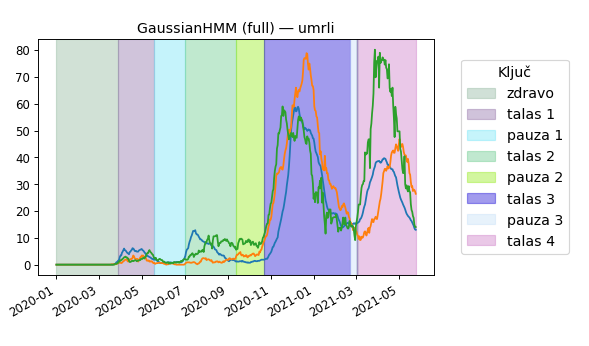
\includegraphics[width=.8\textwidth]{covid.png}
  \caption{Моделовање епидемије \textit{COVID-19} у Србији\cite{vasovic2021}}
  \label{fig:covid}
\end{figure}

Досад је увелико наговештено да су добар избор скривени Марковљеви модели (енгл. \textit{Hidden Markov Model, HMM}), па ће надаље бити речи о њима. Ипак, ваља напоменути да се наведени проблеми још ефектније решавају својеврсним проширењима \textit{HMM}-а, попут условних случајних поља\cite{ponomareva2007} (енгл. \textit{Conditional Random Field, CRF}), или комбинацијом са другим техникама као што су вештачке неуронске мреже\cite{cohen1999} (енгл. \textit{Artificial Neural Network, ANN}).

% ------------------------------------------------------------------------------
\chapter{Моделовање}
% ------------------------------------------------------------------------------
Након мотивације, дошло је време за дефиницију скривених Марковљевих модела, као предложеног решења свих досад изложених проблема. Поред дефиниције, на примеру бацања новчића (непоштене коцкарнице) приказано је како се тачно проблеми моделују помоћу \textit{HMM}, те како се на основу тог модела може одговорити на нека важна питања. Ова глава, дакле, покрива другу петину обрађеног поглавља \textit{Chapter 10: Why Have Biologists Still Not Developed an HIV Vaccine? -- Hidden Markov Models}, и то тачно следеће поднаслове: \textit{Hidden Markov Models}, \textit{The Decoding Problem}, \textit{Finding the Most Likely Outcome of an HMM}, као и преостали део теоријског додатка из \textit{Detours}.

% Hidden Markov Models (1)
\section{Дефиниција модела}
Како би се лакше дошло до општег модела свих досадашњих проблема, а посебно бацања новчића, крупије се, уместо као особа, може схватити као примитивна машина -- аутомат. Структура аутомата за почетак није важна, али његово деловање јесте. Аутомат је секвенцијалне природе, те оперише кроз низ корака. У сваком кораку је у неком приватном стању, које означава који новчић је заправо бачен (конкретно \textit{F} и \textit{B}), при чему јавно приказује исход бацања тог новчића (конкретно \textit{H} и \textit{T}). Стање је, дакле, непознато, па се другачије назива скривеним стањем. И стања и опажања згодно је апстраховати симболима, нпр. баш карактерима, како је и учињено.

У сваком кораку, аутомат доноси две одлуке: у које скривено стање прећи (да ли га променити) и који симбол емитовати у том новом стању. Испоставља се да се обе одлуке могу донети у потпуности стохастички, што би значило да је добијен жељени статистички потковани модел проблема. Заиста, прва одлука може се донети тако што се случајно одабере \textit{F} или \textit{B} као почетно стање (нпр. баш равномерно, са једнаким вероватноћама 1/2), а надаље се у сваком кораку стање мења са неком малом вероватноћом (нпр. 1/10), док се са знатно већом преосталом (нпр. 9/10) остаје у истом стању. Друга одлука доноси се на основу прве и већ познатих вероватносних особина коцкице -- нпр. вероватноћа емитовања \textit{H} једнака је 1/2 у стању \textit{F}, а 3/4 у стању \textit{B}.

Претходно изложени аутомат заправо одговара дуго најављиваном појму скривених Марковљевих модела. \textit{HMM} се традиционално представља као статистички модел који се састоји из следећих основних елемената:
\begin{itemize}
  \item скривених стања $x_i$ -- свако стање из скупа $x$ има индекс $i$,
  \item опажања, опсервација, емисија, приказа, исхода, симбола $y_i$,
  \item полазних вероватноћа $\pi_i$ -- колико је често $x_i$ почетно стање,
  \item вероватноћа прелаза $a_{ij}$ -- колико се често из $x_i$ прелази у $x_j$,
  \item излазних вероватноћа $b_{ij}$ -- колико се често у стању $x_i$ емитује $y_j$.
\end{itemize}
Пример који одговара оваквој дефиницији дат је на слици \ref{fig:hmm}. Наравно, подразумева се да су познати број стања $n$ (тако заправо $x = \{x_1, ..., x_n\}$, $\pi = \{\pi_1, ..., \pi_n\}$ и $a = \{a_{ij}\}_{1 \leq i, j \leq n}$) и број могућих опсервација $m$ (тако заправо $y = \{y_1, ..., y_m\}$ и $b = \{b_{ij}\}_{1 \leq i \leq n, 1 \leq j \leq m}$) као помоћни елементи сваког \textit{HMM}. Како су сви скупови коначни, прецизније се говори о дискретним (мултиномијалним) \textit{HMM}, мада је иначе могуће моделовати разне непрекидне расподеле\cite{jordan2004}.

Како би овакав модел био у потпуности статистички заснован и смислен, обично се захтева да се све појединачне вероватноће сабирају у јединицу: $$\sum_{i=1}^n \pi_i = 1, (\forall i \in \{1, ..., n\}) \sum_{j=1}^m a_{ij} = 1, (\forall i \in \{1, ..., n\}) \sum_{j=1}^m b_{ij} = 1.$$ Постоје, међутим, изузеци који су детаљније обрађени у наставку, када се говори о важним надградњама појма скривених Марковљевих модела.

У овом тренутку је такође значајно нагласити да аутори Компо и Певзнер у уџбенику \textit{Bioinformatics Algorithms} користе нешто другачију нотацију, верну енглеском језику. Наиме, они скуп $x$ означавају као $States$, скуп $y$ као $\Sigma$, матрицу $a_{ij}$ као $transition_{l, k}$, а матрицу $b_{ij}$ као $emission_l(b)$. Такође, потребу за скупом полазних вероватноћа -- који је заправо опционалан, о чему ће бити речи касније -- уводе тек касније, па је \textit{HMM} код њих у основи уређена четворка уместо петорка. Овде је ипак одлучено да се користи познатија нотација, како би читаоцима била лакша употреба повезане литературе. Штавише, \textit{HMM} се у литератури често дефинише још простије, као уређена тројка $\{a, b, \pi\}$, односно $\{A, B, \pi\}$ ако се користе велика слова. Стварно, скупови $x$ и $y$ просто се могу заменити индексима, познатим из наведене тројке.

На основу већ разматране слике \ref{fig:hmm}, познато је да се \textit{HMM} може илустровати \textit{HMM} дијаграмом. У питању је граф чији су чворови стања и опсервације, а гране вероватноће преласка и емисије. Стил је у суштини произвољан, мада се на слици примећује разлика у значењу графичких елемената. Стања су приказана кружним, а емисије квадратним чворовима. Вероватноће преласка исписане су изнад грана, а излазне вероватноће на самим гранама. Прелази и емисије нулте вероватноће (нпр. прелаз са $x_1$ на $x_3$ или на самог себе) нису ни приказани. Други стилови могу приказати све гране, а емисије и вероватноће емисија означити испрекиданим линијама. Независно од стила, \textit{HMM} једнозначно одређује структуру свога дијаграма, а важи и обрнуто.

Сада је могуће искористити \textit{HMM} за прецизно моделовање мотивационог проблема бацања коцкице у непоштеној коцкарници. У конкретном случају, изложеном на почетку поднаслова, уређена петорка изгледа овако:
\begin{itemize}
  \item скривена стања $x = \{F, B\}$ -- нпр. $x_1 = F$ и $x_2 = B$,
  \item опсервације $y = \{H, T\}$ -- нпр. $y_1 = H$ и $y_2 = T$,
  \item полазне вероватноће $\pi = \left\{\dfrac{1}{2}, \dfrac{1}{2}\right\}$ -- нпр. $\pi_1 = P\{x_1\} = P\{F\} = \dfrac{1}{2}$,
  \item преласци $a = \left(\begin{matrix}\dfrac{9}{10} & \dfrac{1}{10}\\[8pt] \dfrac{1}{10} & \dfrac{9}{10}\end{matrix}\right)$ -- нпр. $a_{12} = P\{x_1 \mapsto x_2\} = P\{F \mapsto B\} = \dfrac{1}{10}$,
  \item емисије $b = \left(\begin{matrix}\dfrac{1}{2} & \dfrac{1}{2}\\[8pt] \dfrac{3}{4} & \dfrac{1}{4}\end{matrix}\right)$ -- нпр. $b_{21} = P\{y_1 | x_2\} = P\{H | B\} = \dfrac{3}{4}$.
\end{itemize}
Одговарајући дијаграм приказан је на слици \ref{fig:kock} и пружа исте информације. Служи се истим стилом као претходно описани граф, с тим што додатно испрекидано приказује замишљено полазно стање, што је новина на слици.

\begin{figure}[!ht]
  \centering
  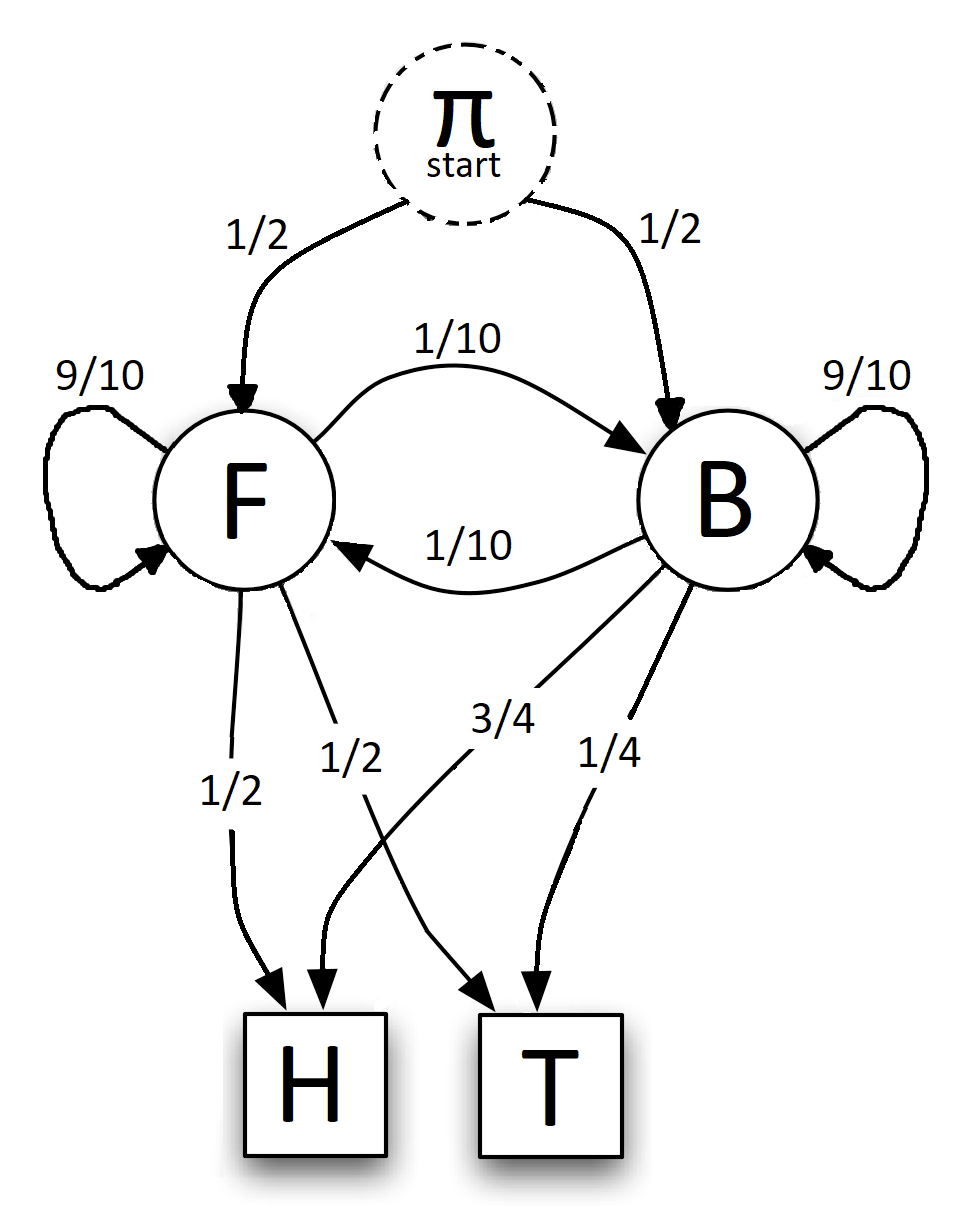
\includegraphics[width=.5\textwidth]{kockarnica.png}
  \caption{Скривени Марковљев модел бацања новчића}
  \label{fig:kock}
\end{figure}

Историјски гледано, појам \textit{HMM} увели су Ленард Баум и сарадници кроз низ статистичких радова објављених у другој половини шездесетих година двадесетог века\cite{baum1966}. У питању је надградња појма Марковљевих ланаца (енгл. \textit{Markov Chain, MC}), који су у суштини \textit{HMM} без емисија. Ради се, дакле, о уобичајеном стохастичком аутомату, који се састоји из стања и вероватноћа прелаза. \textit{MC} је почетком века формулисао руски статистичар Андреј Марков, по коме су и названи, како би моделовао Марковљеве процесе -- стохастичке промене стања такве да тренутно стање зависи искључиво од претходног\cite{markov1906}. Прва практична примена \textit{HMM} била је препознавање говора, док је биолошка примена почела 1986, Бишоповим и Томпсоновим поравнањем \textit{DNA}\cite{bishop1986}.

% Hidden Markov Models (2)
\section{Могућности модела}
Могуће је дефинисати појам скривеног пута $p = p_1...p_k$ као низ $k$ стања кроз која \textit{HMM} пролази, а да притом емитује секвенцу опсервација $o = o_1...o_k$. Примера ради, може бити да је низ видљивих исхода $o = THTHHHTHTTH$, а позадински низ скривених стања $p = FFFBBBBBFFF$. Главна идеја је анализирати у ком су односу $p$ и $o$, те са којом се вероватноћом реализују.

Уз излагање \textit{HMM} за бацање новчића у непоштеној коцкарници, дати су примери значења чланова петорке, који донекле наговештавају могућности скривених Марковљевих модела. Прво, напоменуто је да полазне вероватноће заправо представљају вероватноћу да се у првом кораку ушло у неко стање. Другим речима, то су заправо вероватноће $P\{p\}$ свих могућих једночланих низова скривених стања. Друго, имплицирано је да матрица емисија складишти маргиналну расподелу емисија при познатом стању. У питању су условне вероватноће $P\{o | p\}$ исхода при једночланом низу скривених стања.

Могуће је, дакле, директно из дефиниције \textit{HMM} израчунати вероватноће  $P\{p\}$ и $P\{o | p\}$ за $k = 1$, и то као $P\{x_i\} = \pi_i$, односно $P\{y_j | x_i\} = b_{ij}$. Према познатој формули условне вероватноће, важи $P\{p, o\} = P\{p\} P\{o | p\}$, па је и та вероватноћа тривијално позната за путеве јединичне дужине, као $P\{x_i, y_j\} = \pi_i b_{ij}$. У питању је заједничка вероватноћа да \textit{HMM} пролази кроз низ стања $p$, а да притом емитује управо секвенцу опсервација $o$. Према уобичајеним принципима, могуће је приметити следеће: $\sum_p \sum_o P\{p, o\} = 1$. Наиме, када се саберу вероватноће свих могућих комбинација низа опажања и скривених путева одређене дужине $k$, добија се јединица, што значи да је покривен цео простор догађаја у \textit{HMM}. Из ове дводимензионалне (заједничке) расподеле путева и емисија могу се без проблема извести маргиналне (појединачне) расподеле путева $P\{p\} = \sum_o P\{p, o\}$ и симбола $P\{o\} = \sum_p P\{p, o\}$.

Подсећања ради, оригинални циљ код непоштене коцкарнице био је пронаћи највероватнији низ стања (бачених новчића) за познати низ опсервација (исхода), што је управо максимална вредност $P\{p, o\}$ по свим $p$ за познато $o$. Претходно опште постављен задатак проналаска највероватнијег низа бацања на основу анализе исхода постаје сасвим конкретан статистички проблем -- на основу емитоване ниске симбола $o$ одредити највероватнију секвенцу скривених стања $p$. У наставку је показано како је то заправо могуће урадити.

За почетак, добро је формално дефинисати проблем. Већ је закључено да формулација попут \ref{prob:kock} није добра нити смислена. Зато је и уведен појам \textit{HMM}.

\begin{problem}[H]
  \SetAlgoLined
  \textit{На основу низа исхода бацања новчића, одредити када крупије у непоштеној коцкарници користи који од два могућа новчића.}\\
  \textbf{Улаз}: низ $o = o_1...o_k$ исхода ($H$ и $T$) бацања два новчића ($F$ и $B$).\\
  \textbf{Излаз}: низ $p = p_1...p_k$ новчића такав да је $o_i$ резултат бацања $p_i$.
  \caption{Непоштена коцкарница}
  \label{prob:kock}
\end{problem}

Добра формулација преко појма \textit{HMM} дата је кроз проблем \ref{prob:dekod}. Управо је она детаљно обрађена у наставку овог поглавља, као његов централни део.

\begin{problem}[H]
  \SetAlgoLined
  \textit{Пронаћи оптимални пут кроз \textit{HMM} ако је емитована ниска $o$.}\\
  \textbf{Улаз}: ниска $o = o_1...o_k$ и \textit{HMM}$\{a, b, \pi\}$ који ју је емитовао.\\
  \textbf{Излаз}: скривени пут $p$ који максимизује вероватноћу $P\{p, o\}$ над свим могућим путевима, дакле $\operatorname*{argmax}_p P\{p, o\}$ за улазно $o$.
  \caption{Декодирање приказа}
  \label{prob:dekod}
\end{problem}

Прва идеја јесте исцрпна претрага простора догађаја над маргиналном расподелом $P\{p, o\}$ за познато $o$. Како је $P\{p, o\} = P\{p\} P\{o | p\}$, тако је најзгодније независно израчунати $P\{p\}$ и $P\{o | p\}$ за сваки од $n^k$ скривених путева. Број путева дужине $k$ у \textit{HMM} са $n$ могућих стања је експоненцијалан, јер се одабир своди на варијације -- уређене изборе са понављањем.

Први потпроблем је израчунавање вероватноће пута, што се може формализовати проблемом \ref{prob:put}. Он је у наставку решен у виду једне формуле.

\begin{problem}[H]
  \SetAlgoLined
  \textit{Израчунати вероватноћу скривеног пута $p$ кроз \textit{HMM}.}\\
  \textbf{Улаз}: скривени пут $p = p_1...p_k$ кроз \textit{HMM}$\{a, b, \pi\}$.\\
  \textbf{Излаз}: вероватноћа улазног пута $P\{p\}$.
  \caption{Вероватноћа скривеног пута\cite{ba10a}}
  \label{prob:put}
\end{problem}

Први елемент $P\{p\}$, дакле, представља вероватноћу скривеног пута $p$, односно вероватноћу да \textit{HMM} прође кроз низ стања $p$. Већ је показано да за једночлане путеве важи $P\{x_i\} = \pi_i$. Вишечлани путеви заправо почињу једночланим, а онда се проширују користећи стохастичке прелазе. Стога је $P\{p_1p_2...p_{k-1}p_k\} = P\{p_1\}P\{p_1 \mapsto p_2\}...P\{p_{k-1} \mapsto p_k\}$. Објашњено је већ и да је $P\{x_i \mapsto x_j\} = a_{ij}$, па се свеукупно вероватноћа пута може израчунати као: $$P\{p\} = P\{p_1\} \prod_{i=2}^k P\{p_{i-1} \mapsto p_i\} = \pi_{ind(p_1)} \prod_{i=2}^k a_{ind(p_{i-1}), ind(p_i)}.$$

Други потпроблем је израчунавање вероватноће исхода при познатом путу, што се може формализовати као \ref{prob:ishod}. И то се решава само једном формулом.

\begin{problem}[H]
  \SetAlgoLined
  \textit{Израчунати вероватноћу приказа $o$ на путу $p$ кроз \textit{HMM}.}\\
  \textbf{Улаз}: скривени пут $p = p_1...p_k$ кроз \textit{HMM}$\{a, b, \pi\}$ и ниска $o = o_1...o_k$ која је тим проласком емитована.\\
  \textbf{Излаз}: условна вероватноћа приказа на путу $P\{o | p\}$.
  \caption{Вероватноћа исхода на путу\cite{ba10b}}
  \label{prob:ishod}
\end{problem}

Други елемент $P\{o | p\}$, дакле, представља вероватноћу да \textit{HMM} емитује ниску $o$ при проласку кроз низ стања $p$. Већ је показано да за једночлане путеве важи $P\{y_j | x_i\} = b_{ij}$. Код вишечланих нема разлике, пошто је пут фиксиран и само се прате опсервације. Стога је $P\{o_1...o_k | p_1...p_k\} = P\{o_1 | p_1\}...P\{o_k | p_k\}$. Свеукупно се вероватноћа пута може израчунати као: $$P\{o | p\} = \prod_{i=1}^k P\{o_i | p_i\} = \prod_{i=1}^k b_{ind(p_i), ind(o_i)}.$$

\section{Надградња дефиниције}
Пре коначног решавања проблема декодирања, у дигресији која следи дорађена је дефиниција скривених Марковљевих модела, што доприноси једноставнијем раду са њима. Наиме, како би претходне формуле биле лакше за комбиновање и конкретну имплементацију, добро је на следећи начин надградити \textit{HMM} и сродне појмове попут скривеног пута и низа опсервација:
\begin{itemize}
  \item уводи се експлицитно почетно стање $x_0 = \pi$ уместо одвојених полазних вероватноћа $\pi$, чиме свако $\pi_i$ постаје део матрице прелаза $a_{0i}$,
  \item почетно стање се увек подразумева, као нулти члан скривеног пута, па тако свако $p = p_1...p_k$ постаје $p = p_0p_1...p_k$, и то тако да је $p_0 = x_0$,
  \item уводи се нулта емисија $y_0$, што је заправо празан карактер, чиме се дозвољава да стања буду тиха и не емитују ништа, као почетно стање,
  \item матрице $a_{ij}$ и $b_{ij}$ постају мапе $a_{x_i, x_j}$ и $b_{x_i, y_j}$, што знатно олакшава рад, а исто важи и за низ $\pi_i$, ако се чува (прослеђује), који постаје мапа $\pi_{x_i}$; у вези са тим, из мапа се може прочитати скуп скривених стања и опсервација, чиме се \textit{HMM} дефинитивно своди на тројку $\{a, b, \pi\}$.
\end{itemize}

Оваква дорада свој пун потенцијал показује у напреднијим применама, мада је и њен почетни допринос незанемарљив. Формуле сада постају: $$P\{p\} = \pi_{p_1} \prod_{i=2}^k a_{p_{i-1}, p_i} = \prod_{i=1}^k a_{p_{i-1}, p_i}, P\{o | p\} = \prod_{i=1}^k b_{p_i, o_i}.$$ Заједничка формула вероватноће проласка кроз пут $p$ и приказа $o$ јесте: $$P\{p, o\} = P\{p\} P\{o | p\} = \prod_{i=1}^k a_{p_{i-1}, p_i} \prod_{i=1}^k b_{p_i, o_i} = \prod_{i=1}^k a_{p_{i-1}, p_i} \cdot b_{p_i, o_i}.$$ Интуитивно, заједнички догађај заправо представља низ независних догађаја прелаза и емисија, па је зато $P\{p, o\} = a_{p_0, p_1} b_{p_1, o_1} ... a_{p_{k-1}, p_k} b_{p_k, o_k}$, дакле прелаз из почетног стања у $p_1$, па емисија $o_1$ у $p_1$, затим прелаз из $p_1$ у $p_2$, и тако даље. Све ове формуле дају елегантан начин рачунања само уз помоћ $a$ и $b$.

Ваља искористити прилику и поменути још неке важне надградње \textit{HMM} из литературе, које су у стварности применљивије од основне верзије:
\begin{itemize}
  \item опсервације $y$ могу бити бесконачан скуп, извучене из неке непрекидне расподеле; тада се мапа вероватноћа $b_{ij}$ посматра као мапа расподела $b_i$, која складишти расподеле (густине расподела) емисија стања $x_i$,
  \item само нека стања се означавају као завршна или се уводи експлицитно завршно стање $x_{n+1} = \omega$, што је посебно важно за проблем декодирања,
  \item уместо нестабилних правих вероватноћа користе се логаритамске вероватноће, што ублажава рачунске грешке, мада усложњава алгоритме.
\end{itemize}

Пожељно је усвојити и последњу надградњу, након које формуле постају (подсетник на правило -- логаритам производа је збир логаритама): $$P_{\log}\{p\} = \log P\{p\} = \log \pi_{p_1} + \sum_{i=2}^k \log a_{p_{i-1}, p_i} = \sum_{i=1}^k \log a_{p_{i-1}, p_i},$$ $$P_{\log}\{o | p\} = \log P\{o | p\} = \sum_{i=1}^k \log b_{p_i, o_i},$$ $$P_{\log}\{p, o\} = \log P\{p, o\} = \sum_{i=1}^k (\log a_{p_{i-1}, p_i} + \log b_{p_i, o_i}).$$ Заправо је најефикасније директно радити са логаритамским вероватноћама, односно све вероватноће одмах логаритмовати, укључујући улазне из мапа $a$ и $b$. Под овом претпоставком, формуле су лакше за запис и рачун: $$P_{\log}\{p\} = \pi_{\log, p_1} + \sum_{i=2}^k a_{\log, p_{i-1}, p_i} = \sum_{i=1}^k a_{\log, p_{i-1}, p_i},$$ $$P_{\log}\{o | p\} = \sum_{i=1}^k b_{\log, p_i, o_i}, P_{\log}\{p, o\} = \sum_{i=1}^k (a_{\log, p_{i-1}, p_i} + b_{\log, p_i, o_i}).$$

Надграђени \textit{HMM} сада се може свести на једноставну уређену двојку:
\begin{itemize}
  \item мапа логаритамских вероватоћа прелаза $a_{\log, x_i, x_j}$,
  \item мапа логаритамских излазних вероватноћа $b_{\log, x_i, y_j}$.
\end{itemize}
За конструкцију оваквог објекта треба имати оригинално $a$ и $b$, као и $\pi$, па се зато ипак, интуиције ради, \textit{HMM} и даље званично сматра уређеном тројком $\{a, b, \pi\}$, а не интерно коришћеном трансформисаном двојком $\{a_{\log}, b_{\log}\}$. Згодно је запамтити и следеће вредности као помоћне елементе модела:
\begin{itemize}
  \item скуп скривених стања $x$ и њихов број $n$,
  \item скуп могућих емисија $y$ и њихов број $m$,
  \item мапу логаритамских полазних вероватноћа $\pi_{\log}$,
  \item оригиналне вредности у мапама $a, b, \pi$.
\end{itemize}
Надграђени \textit{HMM} моделује непоштену коцкарницу на следећи начин:
\begin{itemize}
  \item прелази $a_{\log} = \begin{pNiceMatrix}[first-row,first-col] & F & B \\ \pi &\log\dfrac{1}{2} & \log\dfrac{1}{2} \\[8pt] F & \log\dfrac{9}{10} & \log\dfrac{1}{10} \\[8pt] B & \log\dfrac{1}{10} & \log\dfrac{9}{10} \\ \end{pNiceMatrix}$ -- нпр. $a_{\log, F, B} = P_{\log}\{F \mapsto B\}$,
  \item емисије $b_{\log} = \begin{pNiceMatrix}[first-row,first-col] & H & T \\ F &\log\dfrac{1}{2} & \log\dfrac{1}{2} \\[8pt] B & \log\dfrac{3}{4} & \log\dfrac{1}{4} \\ \end{pNiceMatrix}$ -- нпр. $b_{\log, B, H} = P_{\log}\{H |B\} = \log\dfrac{3}{4}$.
\end{itemize}

% The Decoding Problem
\section{Витербијев алгоритам}
Одређивањем формуле $P\{p, o\}$ за путеве произвољне дужине, могуће је приступити проблему максимизације. Како је већ предложено, наивна идеја исцрпне претраге састоји се од генерисања сваког од $n^k$ скривених путева $p$, израчуавања $P\{p, o\}$ за познати низ приказа $o$, и на крају одабира пута који представља $\operatorname*{argmax}_p P\{p, o\}$. Логаритам је монотона трансформација, тако да се задатак не мења ни када се посматрају стабилније вредности $P_{\log}\{p, o\}$, односно важи $\operatorname*{argmax}_p P_{\log}\{p, o\} = \operatorname*{argmax}_p P\{p, o\}$. Из изведене формуле је очигледно да је за свако израчунавање заједничке вероватноће потребно $O(k)$ корака, па је укупна временска сложеност наивног приступа $O(n^k k)$, што је релативно прихватљиво за кратке скривене путеве и мали број стања.

Путеви су, међутим, често врло дугачки, а \textit{HMM} имају велики број скривених стања, те наивни приступ није прихватљив у општем случају. Стога је амерички инжењер електротехнике Ендру Витерби 1967. предложио ефикасније решење\cite{viterbi1967}, засновано на посебном графу, који се може схватити као врста Менхетн графа, појма који је представљен у петом поглављу уџбеника (\textit{Chapter 5: How Do We Compare DNA Sequences? -- Dynamic Programming}). У питању је Витербијев граф, осмишљен на основу основног временског својства сваког Марковљевог модела, а које је представљено на слици \ref{fig:vreme}.

\begin{figure}[!ht]
  \centering
  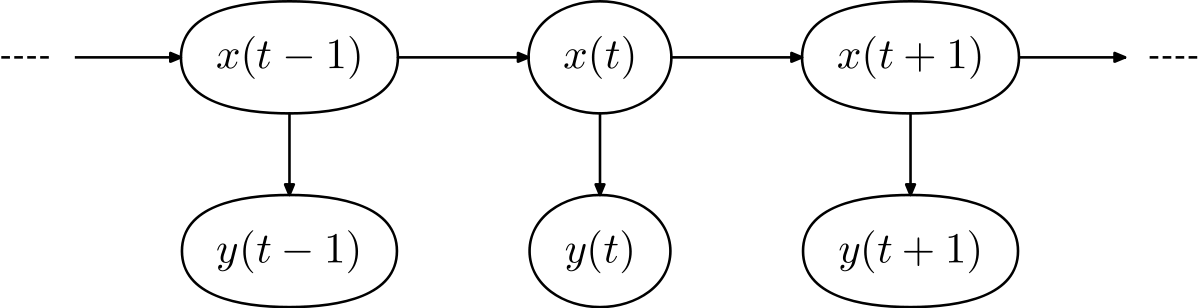
\includegraphics[width=.85\textwidth]{vreme.png}
  \caption{Ток времена код скривених Марковљевих модела\cite{vreme}}
  \label{fig:vreme}
\end{figure}

Сваки \textit{HMM}, наиме, моделује један Марковљев процес, што је поменуто при дефиницији. Последица је да тренутно стање зависи искључиво од претходног на путу и ниједног другог -- мапа $a$ моделује $p_{t-1} \mapsto p_t$, у ознакама са слике $x(t-1) \mapsto x(t)$. Исто тако, опсервација зависи искључиво од текућег стања -- мапа  $b$ моделује $p_t \mapsto o_t$, у ознакама са слике $x(t) \mapsto y(t)$. Стога се \textit{HMM} понекад дефинише и нешто другачије, као уређени пар $\{X, Y\}$, где је $X$ систем који се моделује, а $Y$ процес чије понашање директно зависи од $X$.

Прецизније, $X$ је Марковљев процес са неопсервабилним ("скривеним") стањима ($x$ из дефиниције), а циљ модела је да се нешто о том процесу сазна на основу опажања ($y$ из дефиниције) процеса $Y$, чије је понашање видљиво. Притом условна расподела $Y$ (на слици конкретна вредност $y(t)$, а у низу опсервација приказ $o_t$) у неком временском тренутку $t$ (индекс низа) зависи искључиво од стања $X$ у том истом тренутку (на слици конкретна вредност $x(t)$, а на скривеном путу стање $p_t$). Приметно је да је ова дефиниција у суштини једнака претходно изложеним, с тим што је математички напреднија (захтевнија) -- углавном је теже разумети торку апстрактних статистичких процеса него једноставних структура попут скупова, низова, матрица и мапа. На конкретном примеру непоштене коцкарнице, $X$ је процес одабира (замене) новчића, а $Y$ процес бацања новчића, односно добијања исхода тог бацања.

Све у свему, описано временско својство оправдава употребу Витербијевог графа, чији је пример за проблем непоштене коцкарнице дат на слици \ref{fig:kockvit}. Граф се састоји из мреже (матрице) чворова чија основа има $n$ редова и $k$ колона. Свака колона састоји се од низа чворова који представљају сва скривена стања у тренутку $t$. Из сваког чвора у колони $t-1$ усмерена је по једна грана у сваки чвор из колоне $t$, на основу чињенице да се из сваког стања у тренутку $t-1$ може прећи у било које стање у тренутку $t$. Поред ове основе, мрежа има и два посебна чвора -- извор (експлицитно почетно стање) и понор (експлицитно завршно стање). Замисао овакве мреже је да истовремено моделује све скривене путеве дужине $k$ кроз \textit{HMM} са $n$ скривених стања.

\begin{figure}[!ht]
  \centering
  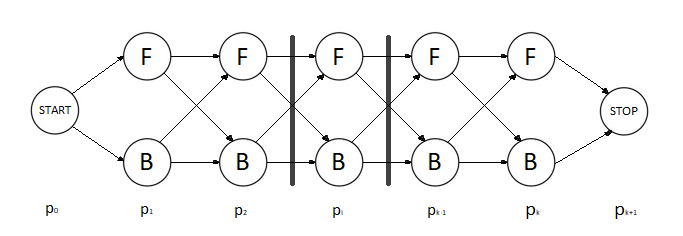
\includegraphics[width=\textwidth]{kock_graf.png}
  \caption{Витербијев граф непоштене коцкарнице}
  \label{fig:kockvit}
\end{figure}

Стварно, различитих путева од извора до понора има тачно $n^k$, и сваки одговара једном скривеном путу у \textit{HMM}. Остаје још питање како отежати гране Витербијевог графа, након чега се он може искористити за проблем максимизације кумулативне тежине у понору. То је заправо основни проблем над сваким Менхетном, који се може решити алгортмима из петог поглавља.

За хватање интуиције у вези са моћи Витербијевог графа, није лоше увести проблем \ref{prob:maxput}. Задатак је пронаћи највероватнији скривени пут дужине $k$.

\begin{problem}[H]
  \SetAlgoLined
  \textit{Израчунати највероватнији скривени пут $p$ кроз \textit{HMM}.}\\
  \textbf{Улаз}: дужина $k$ скривеног пута кроз \textit{HMM}$\{a, b, \pi\}$.\\
  \textbf{Излаз}: највероватнији скривени пут $p = p_1...p_k$.
  \caption{Највероватнији скривени пут}
  \label{prob:maxput}
\end{problem}

Наивно решење проблема своди се на већ разматрану исцрпну претрагу простора скривених путева, којих је $n^k$. Вероватноћа сваког пута рачуна се у $O(k)$ корака, па је временска сложеност експоненцијална $O(n^k k)$. Ипак, могуће је искористити Витербијев граф како би се постигло знатно побољшање.

Нека је мрежа чворова представљена мапом $s$, таквом да $s_{x_i, t}$ складишти неки податак о чвору (стању) $x_i$ у тренутку $t$. Оваква структура погодна је за свођење полазног проблема на проблем динамичког програмирања. Како је крајњи циљ максимизација вероватноће пута, нека $s_{x_i, t}$ заправо складишти вероватноћу оптималног пута дужине $t$ који се завршава у стању $x_i$. Очигледно, за путеве јединичне дужине, односно у тренутку $t=1$, важи: $$s_{x_i, 1} = P\{x_i\} = \pi_{x_i} = a_{\pi, x_i}.$$

Испоставља се да се и остале тежине могу узети из матрице прелаза, што важи због темпоралног својства Марковљевих процеса. Како свако стање зависи искључиво од првог претходног, тако се и вероватноћа нејединичног пута може максимизовати тако што се размотре сва могућа претходна стања, односно за једно стање краћи путеви. Тако је рекурентна формула: $$s_{x_i, t} = \max_j \{s_{x_j, t-1} \cdot a_{x_j, x_i}\},$$ $$P\{p_{opt}\} = \max_p P\{p\} = \max_j \{s_{x_j, k}\}.$$ Наравно, проблеми са рачуном се решавају логаритамском трансформацијом: $$s_{\log, x_i, 1} = P_{\log}\{x_i\} = \pi_{\log, x_i} = a_{\log, \pi, x_i},$$ $$s_{\log, x_i, t} = \max_j \{s_{\log, x_j, t-1} + a_{\log, x_j, x_i}\},$$ $$P_{\log}\{p_{opt}\} = \max_p P_{\log}\{p\} = \max_j \{s_{\log, x_j, k}\}.$$ Ова верзија је боља и због тога што су Менхетн алгоритми адитивни по природи, односно засновани су на сабирању, а не множењу вредности. Слика \ref{fig:tribac} приказује како Витербијев граф моделује три бацања у непоштеном казину.

\begin{figure}[!ht]
  \centering
  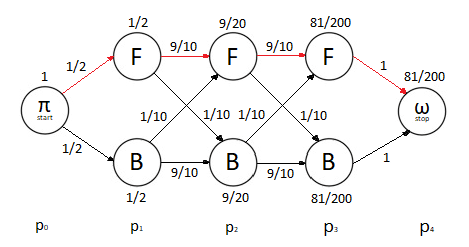
\includegraphics[width=.9\textwidth]{tri_bacanja.png}
  \caption{Максимизација $P\{p\}$ са три бацања}
  \label{fig:tribac}
\end{figure}

Општи облик ове рекурентне релације заправо је заснован на тежинама грана $\tau$, где мапа облика $\tau_{x_i, x_j, t}$ означава тежину гране из чвора $x_i$ ка $x_j$ у тренитку $t$, укључујући експлицитни почетни извор $\pi$ и завршни понор $\omega$. Оне су у конкретном случају биле логаритми вероватноћа преласка или саме вероватноће, као на слици, у ком случају се множи уместо сабира: $$s_{x_i, 1} = \tau_{\pi, x_i}, s_{x_i, t} = \max_j \{s_{x_j, t-1} + \tau_{x_j, x_i, t}\},$$ $$P\{p_{opt}\} = \max_p P\{p\} = \max_j \{s_{x_j, k} + \tau_{x_j, \omega}\}.$$

Како је моделовано $P\{p\}$, тако се може моделовати и $P\{p, o\}$ за фиксирано $o$. У првом случају, важило је $\tau_{x_i, x_j, t} = \tau_{x_i, x_j} = a_{x_i, x_j}$, док је у другом нешто сложеније $\tau_{x_i, x_j, t} = a_{x_i, x_j} \cdot b_{x_j, o_t}$, дакле вероватноћа догађаја да \textit{HMM} пређе из стања $x_i$ у стање $x_j$, након чега емитује симбол $o_t$. Формуле су сада: $$s_{x_i, 1} = \pi_{x_i} \cdot b_{x_i, o_1} = a_{\pi, x_i} \cdot b_{x_i, o_1},$$ $$s_{x_i, t} = \max_j \{s_{x_j, t-1} \cdot a_{x_j, x_i} \cdot b_{x_i, o_t}\},$$ $$P\{p_{opt}, o\} = \max_p P\{p, o\} = \max_j \{s_{x_j, k}\}.$$ Једнаке су и логаритамске верзије, па се оне не наводе као можда сувишне.

Када је у питању проблем максимизације, могуће је моделовати и $P\{o | p\}$, с тим што за то није неопходан Витербијев граф. Поставка \ref{prob:maxops} је у наставку.

\begin{problem}[H]
  \SetAlgoLined
  \textit{Израчунати највероватнији низ емисија на путу $p$ кроз \textit{HMM}.}\\
  \textbf{Улаз}: скривени пут $p = p_1...p_k$ кроз \textit{HMM}$\{a, b, \pi\}$.\\
  \textbf{Излаз}: највероватнија опажања $o = o_1...o_k$ на путу $p$.
  \caption{Највероватније опсервације на путу}
  \label{prob:maxops}
\end{problem}

Формула максималне вероватноће је једноставна, по свакој опсервацији: $$P\{o_{opt} | p\} = \prod_{i=1}^k \max_j b_{p_i, y_j}.$$

Претходно изложени систем рада са \textit{HMM}, заснован на Витербијевог графу и динамичком програмирању назива се Витербијев алгоритам\cite{ba10c}, посебно када се примењује на декодирање -- проблем \ref{prob:dekod}. Изведеним рекурентним формулама једино треба додати систем путоказа, како би поред вероватноће оптималног пута могао бити добијен (реконструисан) и сам највероватнији пут.

Важна предност Витербијевог алгоритма је његова сложеност. Основна мрежа графа има $nk$ чворова и $n^2 (k-1)$ грана (из свих $n$ стања ка свим $n$ стањима у $k-1$ временском прелазу), чему се додају још два додатна чвора и $2n$ грана повезаних са тим чворовима. Израчунавање иде по чворовима, користећи гране, тако да је укупна временска и просторна сложеност $O(n^2 k)$ уколико би се користио експлицитни граф. Ово је временски знатно боље од наивних $O(n^k k)$, али је просторно захтевније, јер наивни приступ захтева само $O(k)$ помоћног простора. У многим случајевима је, међутим, граф довољно само замислити, а у раду користити искључиво мапу $s$ и путоказе, не и тежине $\tau$, што за собом повлачи нешто бољу просторну сложеност $O(nk)$.

У стварности је могуће добити још бољу сложеност. Наиме, многи \textit{HMM} имају забрањене прелазе између неких стања. Таква ситуација веома је честа, а приказана је још на уводној слици \ref{fig:hmm}. Могуће је без проблема уклонити гране Витербијевог графа које одговарају таквим прелазима, што знатно смањује време извршавања алгоритма. Посебно занимљиви могу бити недозвољени прелази који укључују извор и понор. На тај начин се може онемогућити да неко стање буде полазно или завршно, што често има биолошки смисао.

% Finding the Most Likely Outcome of an HMM
\section{Алгоритам "напред"}
Сваки \textit{HMM}, подсећања ради, може се схватити као уређени пар два процеса -- скривеног Марковљевог који се очитава скривеним путем $p$ и опсервабилног зависног који се очитава низом емисија $o$. Цела идеја \textit{HMM} јесте детаљно статистички потковано моделовање тих процеса и њиховог односа.

Досад је било речи о појединачној расподели $P\{p\}$, условној $P\{o | p\}$ и заједничкој $P\{p, o\}$. Могуће је моделовати и појединачну расподелу $P\{o\}$, а затим и условну $P\{p | o\}$, на основу познате формуле $P\{p, o\} = P\{o\} P\{p | o\}$. Основни задатак из овог домена модела дат је кроз проблем \ref{prob:ops}. Потребно је израчунати вероватноћу да \textit{HMM} емитује неки низ симбола дужине $k$.

\begin{problem}[H]
  \SetAlgoLined
  \textit{Израчунати вероватноћу приказа $o$ у \textit{HMM}.}\\
  \textbf{Улаз}: низ опажања $o = o_1...o_k$ у \textit{HMM}$\{a, b, \pi\}$.\\
  \textbf{Излаз}: вероватноћа улазног низа опажања $P\{o\}$.
  \caption{Вероватноћа опсервација\cite{ba10d}}
  \label{prob:ops}
\end{problem}

Још једном, наивни приступ састоји се од генерисања свих $n^k$ путева и сумирања вероватноћа на њима, према раније изложеној маргинализацији $P\{o\} = \sum_p P\{p, o\}$. Занимљиво је, међутим, приметити да је ова маргинализација врло слична садржају мапе $s$ код Витербијевог алгоритма, која у понору израчунава $P\{p_{opt}, o\} = \max_p P\{p, o\}$. Једина разлика је у примењеном оператору -- да ли је сума или максимум. Ово није случајно, јер је идеја обе формуле обилазак свих скривених путева кроз \textit{HMM} истовремено.

Све у свему, сасвим је оправдано увести нову мапу $f$ (од енгл. \textit{forward} -- напред), надахнуту претходном $s$ (од енгл. \textit{score} -- скор), такву да елемент $f_{x_i, t}$ складишти вероватноћу префикса опажања дужине $t$ (подниз $o_1...o_t$), насталог на скривеном путу који завршава стањем $x_i$. Одатле су формуле: $$f_{x_i, 1} = \pi_{x_i} \cdot b_{x_i, o_1} = a_{\pi, x_i} \cdot b_{x_i, o_1},$$ $$f_{x_i, t} = \sum_j s_{x_j, t-1} \cdot a_{x_j, x_i} \cdot b_{x_i, o_t},$$ $$P\{o\} = \sum_j s_{x_j, k}.$$ Као и досад, логаритамске верзије производе мењају збировима. Овога пута има и један додатак: сума се мења посебним оператором $\operatorname{logsumexp}_j f(j)$, који моделује сабирање у логаритамском домену -- апроксимира $\log \sum_j e^{f(j)}$.

За крај, ваља поменути и сродан проблем одређивања највероватнијег исхода, односно $\operatorname{argmax}_o P\{o\}$. И овде је наивно решење сувише неефикасно. Напредније се имплементира помоћу тродимензионог Витербијевог графа, који применом оба оператора успешно максимизује суму $\max_o \sum_p P\{p, o\}$.

% ------------------------------------------------------------------------------
\chapter{Биолошки значај}
% ------------------------------------------------------------------------------
Након дефинисања скривених Марковљевих модела, описа њихове примене и алгоритама који дају одговоре на важна питања у вези са моделованим проблемом, ред је да се непосредно опише биолошки значај \textit{HMM}, односно њихова примена у досад изложеним биоинформатичким проблемима. Конкретно, глава која следи бави се потрагом за генима, односно откривањем \textit{CG} острва помоћу \textit{HMM}, као и употребом профилних \textit{HMM} за решавање проблема попут откривања фенотипа \textit{HIV}-а. Она, дакле, покрива трећу и четврту петину обрађеног поглавља \textit{Chapter 10: Why Have Biologists Still Not Developed an HIV Vaccine? -- Hidden Markov Models}, и то тачно поднаслове \textit{Profile HMMs for Sequence Alignment} и \textit{Classifying proteins with profile HMMs}.

\section{Потрага за генима}
...

% Profile HMMs for Sequence Alignment
% Classifying proteins with profile HMMs
\section{Профилни модели}
...

% ------------------------------------------------------------------------------
\chapter{Учење модела}
% ------------------------------------------------------------------------------
% Learning the Parameters of an HMM
% Soft Decisions in Parameter Estimation
% Baum-Welch Learning
За крај, прича о скривеним Марковљевим моделима допуњује се још једном важном особином \textit{HMM} -- способношћу (машинског) учења поткрепљивањем. Досад је било речи о већ готовим моделима, али прави потенцијал \textit{HMM} показују тек онда када се сви параметри модела науче, уместо да се хардкодирају. Ова глава, дакле, покрива последњу петину обрађеног поглавља \textit{Chapter 10: Why Have Biologists Still Not Developed an HIV Vaccine? -- Hidden Markov Models}, и то тачно следеће поднаслове: \textit{Learning the Parameters of an HMM}, \textit{Soft Decisions in Parameter Estimation} и \textit{Baum-Welch Learning}.

% ------------------------------------------------------------------------------
% The Many Faces of HMMs
% Epilogue: Nature is a Tinkerer and not an Inventor
% Bibliography Notes
\chapter{Закључак}
% ------------------------------------------------------------------------------
Досад је изложен појам скривених Марковљевих модела, као и њихов биоинформатички значај. Дата је детаљна мотивација за увођење статистички потованог аутомата, након чега је појам \textit{HMM} разрађен на мотивационом примеру непоштене коцкарнице (бацање два новчића). Затим је и примењен на решавање важних биолошких проблема, попут проналажења \textit{CG} острва (места са генима) и напредног бављења генским и протеинским профилима.

У последњој глави овог рада су надаље сумиране информације из закључних поднаслова обрађеног поглавља \textit{Chapter 10: Why Have Biologists Still Not Developed an HIV Vaccine? -- Hidden Markov Models}, и то тачно \textit{The Many Faces of HMMs} и \textit{Epilogue: Nature is a Tinkerer and not an Inventor}, мада су поменути и додатни подаци из помоћног поднаслова \textit{Bibliography Notes}.

Значајна напредна примена \textit{HMM} која превазилази оквире уџбеника јесте моделовање отпорности \textit{HIV}-а на лекове. У уводној мотивацији поменуто је да се заражени пацијенти лече коктелом антивирусних лекова, који је због високе стопе мутација често посебно осмишљен за сваког појединца, како би терапија била успешна. Мутације могу да онеспособе дејство неког лека који је раније имао ефекта. Стога је разумевање отпорности од високог значаја. Нико Беренвинкел и Матијас Дртон су 2006. предложили модел реактивности соја на лекове заснован баш на \textit{HMM}, додуше изразито комплексном\cite{beerenwinkel2007}.

Када су протеини у питању, ваља напоменути да се они у суштини састоје из више повезаних целина које се називају доменима. Домени могу бити различитих структура и функција, и управо се они чешће анализирају него цели протеини. Године 2002. Бејтман и сарадници описали су употребу профилних \textit{HMM}, на основу чега је осмишљена позната база података Пфам\cite{bateman2002}. Она се данас састоји од скоро 20.000 вишеструких поравнања разних протеинских домена и рутински се користи у анализи нових протеинских секвенци\cite{pfam}.

Све у свему, скривени Марковљеви модели прешли су дуг пут од својих првих употреба у рачунарској биологији (нпр. Черчил 1989\cite{churchill1989}, Крог и сарадници 1994\cite{krogh1994}, Балди и сарадници 1994\cite{baldi1994}) до данашње широке биоинформатичке примене. Поменута је употреба \textit{HMM} за моделовање и препознавање људског понашања, гестова, рукописа и говора, обраду звука и сигнала, одређивање врсте речи у тексту или чак моделовање тока пандемије \textit{COVID-19} у Републици Србији засновано на најосновнијим подацима, као на слици \ref{fig:covid}. Објашњен је значај \textit{HMM} како код проблема надгледаног, тако и код проблема ненадгледаног машинског учења. Наведене су многе могућности \textit{HMM}, укључујући способност учења свих параметара модела поткрепљивањем.

Паралелно са писањем овог текста, направљен је електронски уџбеник, као суштински најзначајнији допринос рада. Уџбеник је реализован у виду \textit{Jupyter} свезака, које су заједно са свим осталим материјалима доступне на \textit{GitHub}-у\cite{vasovich2021}. Концепт је такав да свеске садрже једнак текст као у писаном раду, али успут складиште и \textit{Python} кодове који имплементирају у тексту изложене алгоритме. Имплементирана су сва предложена решења из књиге \textit{Bioinformatics Algorithms}, али и многа друга. Како се кодови интерпретирају, они су у потпуности интерактивни и могу лако послужити за самосталан студентски рад и детаљније упознавање са имплементацијама. За случај да читаоцу нису доступни \textit{Python} интерпретатор и/или \textit{Jupyter} сервер, направљена је и \textit{HTML} верзија материјала, која, додуше, није интерактивна.

Свеукупно, обрађена лекција електронског уџбеника доприноси усвајању знања о скривеним Марковљевим моделима и њиховој примени у биоинформатици, независно од тога да ли читалац слуша мастер курс Увод у биоинформатику на Математичком факултету Универзитета у Београду. За разумевање је неопходно само основно предзнање из математике (углавном вероватноће) и биологије (улавном генетике), што је ниво средње школе. Било би добро да иницијатива у оквиру које уџбеник настаје заживи, те да у најскоријем року свака лекција буде доступна у потпуности у електронском облику.

% ------------------------------------------------------------------------------
% Literatura
% ------------------------------------------------------------------------------
\literatura

\end{CJK}
\end{document}